\begin{figure}
\begin{center}
\psset{unit=1.5cm} % 12cm width / 8 figures = 1.5cm
\addtolength{\subfigbottomskip}{-1.5cm}
\multido{\ix=0+1}{13}{ % first 13
\setcounter{subfigure}{0}
 \subfigure{
  \begin{pspicture}(-0.25,0)(-0.05,1)
   \input{common/permute\ix}
  \end{pspicture}
  \includegraphics[width=12.0cm]{primarystripes/\ix.eps}
  \rput[cl](0.05,0.5){\ix}
 }
}
\subfigure{ % last one with labels
  \begin{pspicture}(-0.25,0)(-0.05,1)
   \psframe[](-0.25,0.01)(-0.05,0.25)
\psframe[fillcolor=gray,fillstyle=solid](-0.25,0.25)(-0.05,0.5)
\psframe[fillcolor=gray,fillstyle=solid](-0.25,0.5)(-0.05,0.75)
\psframe[fillcolor=gray,fillstyle=solid](-0.25,0.75)(-0.05,0.99)

  \end{pspicture}
  
\includegraphics[width=12.0cm]{primarystripes/14.eps}
  \rput[cl](0.05,0.5){14}
  \psset{unit=1.5cm}
  \rput[ct](-0.55,-0.3){$\frac{7\pi}{4}$}
  \rput[ct](-1.55,-0.3){$\frac{6\pi}{4}$}
  \rput[ct](-2.55,-0.3){$\frac{5\pi}{4}$}
  \rput[ct](-3.55,-0.3){$\pi$}
  \rput[ct](-4.55,-0.3){$\frac{3\pi}{4}$}
  \rput[ct](-5.55,-0.3){$\frac{\pi}{2}$}
  \rput[ct](-6.55,-0.3){$\frac{\pi}{4}$}
  \rput[ct](-7.55,-0.3){$0$}
 }
 \end{center}
\caption{Permutations of the Monte Carlo simulation around the ring:
intensity and phase.  Intensity values have been normalized for each frame
while phase values normalized across the entire dataset.}
\label{fig:clevergridlinhsv}
\end{figure}

\begin{figure}
\begin{center}
\psset{unit=1.5cm}
\addtolength{\subfigbottomskip}{-1.5cm}
\multido{\ix=0+1}{13}{
\setcounter{subfigure}{0}
 \subfigure{
  \begin{pspicture}(-0.25,0)(-0.05,1)
   \input{common/permute\ix}
  \end{pspicture}
  % this file name sucks because of the dot, but too lazy to change
  \includegraphics[width=12.0cm]{primarystripes/\ix.-intensity.eps}
  \rput[cl](0.05,0.5){\ix}
 }
}
\subfigure{
  \begin{pspicture}(-0.25,0)(-0.05,1)
   \psframe[](-0.25,0.01)(-0.05,0.25)
\psframe[fillcolor=gray,fillstyle=solid](-0.25,0.25)(-0.05,0.5)
\psframe[fillcolor=gray,fillstyle=solid](-0.25,0.5)(-0.05,0.75)
\psframe[fillcolor=gray,fillstyle=solid](-0.25,0.75)(-0.05,0.99)

  \end{pspicture}
  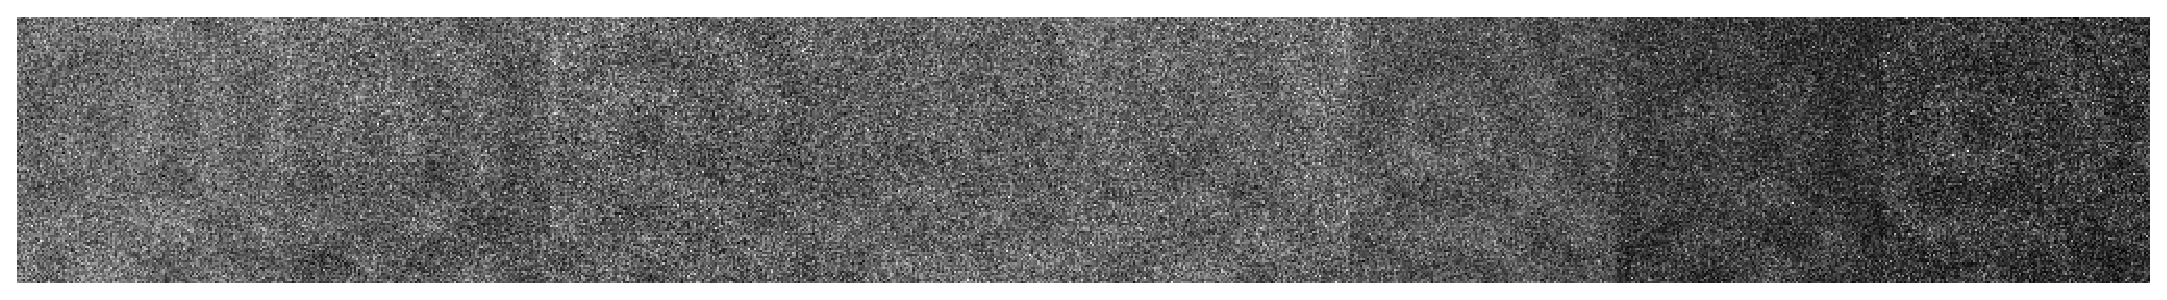
\includegraphics[width=12.0cm]{primarystripes/14.-intensity.eps}
  \rput[cl](0.05,0.5){14}
  \psset{unit=1.5cm}
  \rput[ct](-0.55,-0.3){$\frac{7\pi}{4}$}
  \rput[ct](-1.55,-0.3){$\frac{6\pi}{4}$}
  \rput[ct](-2.55,-0.3){$\frac{5\pi}{4}$}
  \rput[ct](-3.55,-0.3){$\pi$}
  \rput[ct](-4.55,-0.3){$\frac{3\pi}{4}$}
  \rput[ct](-5.55,-0.3){$\frac{\pi}{2}$}
  \rput[ct](-6.55,-0.3){$\frac{\pi}{4}$}
  \rput[ct](-7.55,-0.3){$0$}
 }
\end{center}
\caption{Permutations of the Monte Carlo simulation around the ring:
intensity only.  Intensity values have been normalized for each frame
individually.}
\label{fig:clevergridlinintensity}
\end{figure}


% probability distribution function around the ring
\begin{figure}
\begin{center}
\addtolength{\subfigbottomskip}{-1cm}
\psset{yAxisLabel=,xAxisLabel=,yAxis=false}
\multido{\ix=0+1}{13}{%
\setcounter{subfigure}{0}
\subfigure{
 \psset{unit=40.75pt}
 \begin{pspicture}(-0.25,0)(-0.05,1)
 \input{common/permute\ix}
 \end{pspicture}
  \begin{psgraph}[Dx=0.1,labels=none](0,0)(1,0.08){14cm}{1.5cm}
  \psset{fillstyle=solid,fillcolor=red}
  \input{stats/ringpdf\ix}
 \end{psgraph}
 }
}
\subfigure{
 \psset{unit=40.75pt}
 \begin{pspicture}(-0.25,0)(-0.05,1)
 \psframe[](-0.25,0.01)(-0.05,0.25)
\psframe[fillcolor=gray,fillstyle=solid](-0.25,0.25)(-0.05,0.5)
\psframe[fillcolor=gray,fillstyle=solid](-0.25,0.5)(-0.05,0.75)
\psframe[fillcolor=gray,fillstyle=solid](-0.25,0.75)(-0.05,0.99)

 \end{pspicture}
  \begin{psgraph}[Dx=0.1](0,0)(1,0.08){14cm}{1.5cm}
  \psset{fillstyle=solid,fillcolor=red}
  \psframe(0.000000,0)(0.005000,0.036111)
\psframe(0.005000,0)(0.010000,0.022222)
\psframe(0.010000,0)(0.015000,0.019444)
\psframe(0.015000,0)(0.020000,0.027778)
\psframe(0.020000,0)(0.025000,0.030556)
\psframe(0.025000,0)(0.030000,0.016667)
\psframe(0.030000,0)(0.035000,0.030556)
\psframe(0.035000,0)(0.040000,0.019444)
\psframe(0.040000,0)(0.045000,0.022222)
\psframe(0.045000,0)(0.050000,0.033333)
\psframe(0.050000,0)(0.055000,0.025000)
\psframe(0.055000,0)(0.060000,0.011111)
\psframe(0.060000,0)(0.065000,0.016667)
\psframe(0.065000,0)(0.070000,0.011111)
\psframe(0.070000,0)(0.075000,0.016667)
\psframe(0.075000,0)(0.080000,0.019444)
\psframe(0.080000,0)(0.085000,0.005556)
\psframe(0.085000,0)(0.090000,0.025000)
\psframe(0.090000,0)(0.095000,0.027778)
\psframe(0.095000,0)(0.100000,0.011111)
\psframe(0.100000,0)(0.105000,0.002778)
\psframe(0.105000,0)(0.110000,0.016667)
\psframe(0.110000,0)(0.115000,0.011111)
\psframe(0.115000,0)(0.120000,0.019444)
\psframe(0.120000,0)(0.125000,0.005556)
\psframe(0.125000,0)(0.130000,0.008333)
\psframe(0.130000,0)(0.135000,0.011111)
\psframe(0.135000,0)(0.140000,0.011111)
\psframe(0.140000,0)(0.145000,0.011111)
\psframe(0.145000,0)(0.150000,0.011111)
\psframe(0.150000,0)(0.155000,0.013889)
\psframe(0.155000,0)(0.160000,0.011111)
\psframe(0.160000,0)(0.165000,0.008333)
\psframe(0.165000,0)(0.170000,0.008333)
\psframe(0.170000,0)(0.175000,0.011111)
\psframe(0.175000,0)(0.180000,0.011111)
\psframe(0.180000,0)(0.185000,0.005556)
\psframe(0.185000,0)(0.190000,0.002778)
\psframe(0.190000,0)(0.195000,0.008333)
\psframe(0.195000,0)(0.200000,0.011111)
\psframe(0.200000,0)(0.205000,0.011111)
\psframe(0.205000,0)(0.210000,0.008333)
\psframe(0.210000,0)(0.215000,0.011111)
\psframe(0.215000,0)(0.220000,0.011111)
\psframe(0.220000,0)(0.225000,0.005556)
\psframe(0.225000,0)(0.230000,0.005556)
\psframe(0.230000,0)(0.235000,0.005556)
\psframe(0.235000,0)(0.240000,0.005556)
\psframe(0.240000,0)(0.245000,0.013889)
\psframe(0.245000,0)(0.250000,0.002778)
\psframe(0.250000,0)(0.255000,0.013889)
\psframe(0.255000,0)(0.260000,0.011111)
\psframe(0.260000,0)(0.265000,0.005556)
\psframe(0.265000,0)(0.270000,0.000000)
\psframe(0.270000,0)(0.275000,0.000000)
\psframe(0.275000,0)(0.280000,0.002778)
\psframe(0.280000,0)(0.285000,0.002778)
\psframe(0.285000,0)(0.290000,0.008333)
\psframe(0.290000,0)(0.295000,0.008333)
\psframe(0.295000,0)(0.300000,0.005556)
\psframe(0.300000,0)(0.305000,0.008333)
\psframe(0.305000,0)(0.310000,0.002778)
\psframe(0.310000,0)(0.315000,0.005556)
\psframe(0.315000,0)(0.320000,0.005556)
\psframe(0.320000,0)(0.325000,0.005556)
\psframe(0.325000,0)(0.330000,0.008333)
\psframe(0.330000,0)(0.335000,0.002778)
\psframe(0.335000,0)(0.340000,0.005556)
\psframe(0.340000,0)(0.345000,0.002778)
\psframe(0.345000,0)(0.350000,0.008333)
\psframe(0.350000,0)(0.355000,0.002778)
\psframe(0.355000,0)(0.360000,0.005556)
\psframe(0.360000,0)(0.365000,0.002778)
\psframe(0.365000,0)(0.370000,0.002778)
\psframe(0.370000,0)(0.375000,0.005556)
\psframe(0.375000,0)(0.380000,0.000000)
\psframe(0.380000,0)(0.385000,0.000000)
\psframe(0.385000,0)(0.390000,0.002778)
\psframe(0.390000,0)(0.395000,0.000000)
\psframe(0.395000,0)(0.400000,0.008333)
\psframe(0.400000,0)(0.405000,0.002778)
\psframe(0.405000,0)(0.410000,0.002778)
\psframe(0.410000,0)(0.415000,0.005556)
\psframe(0.415000,0)(0.420000,0.002778)
\psframe(0.420000,0)(0.425000,0.002778)
\psframe(0.425000,0)(0.430000,0.002778)
\psframe(0.430000,0)(0.435000,0.002778)
\psframe(0.435000,0)(0.440000,0.000000)
\psframe(0.440000,0)(0.445000,0.000000)
\psframe(0.445000,0)(0.450000,0.000000)
\psframe(0.450000,0)(0.455000,0.000000)
\psframe(0.455000,0)(0.460000,0.005556)
\psframe(0.460000,0)(0.465000,0.000000)
\psframe(0.465000,0)(0.470000,0.000000)
\psframe(0.470000,0)(0.475000,0.002778)
\psframe(0.475000,0)(0.480000,0.005556)
\psframe(0.480000,0)(0.485000,0.002778)
\psframe(0.485000,0)(0.490000,0.002778)
\psframe(0.490000,0)(0.495000,0.000000)
\psframe(0.495000,0)(0.500000,0.000000)
\psframe(0.500000,0)(0.505000,0.005556)
\psframe(0.505000,0)(0.510000,0.008333)
\psframe(0.510000,0)(0.515000,0.000000)
\psframe(0.515000,0)(0.520000,0.008333)
\psframe(0.520000,0)(0.525000,0.002778)
\psframe(0.525000,0)(0.530000,0.002778)
\psframe(0.530000,0)(0.535000,0.000000)
\psframe(0.535000,0)(0.540000,0.000000)
\psframe(0.540000,0)(0.545000,0.000000)
\psframe(0.545000,0)(0.550000,0.002778)
\psframe(0.550000,0)(0.555000,0.002778)
\psframe(0.555000,0)(0.560000,0.000000)
\psframe(0.560000,0)(0.565000,0.000000)
\psframe(0.565000,0)(0.570000,0.005556)
\psframe(0.570000,0)(0.575000,0.002778)
\psframe(0.575000,0)(0.580000,0.000000)
\psframe(0.580000,0)(0.585000,0.002778)
\psframe(0.585000,0)(0.590000,0.000000)
\psframe(0.590000,0)(0.595000,0.002778)
\psframe(0.595000,0)(0.600000,0.000000)
\psframe(0.600000,0)(0.605000,0.002778)
\psframe(0.605000,0)(0.610000,0.000000)
\psframe(0.610000,0)(0.615000,0.002778)
\psframe(0.615000,0)(0.620000,0.002778)
\psframe(0.620000,0)(0.625000,0.000000)
\psframe(0.625000,0)(0.630000,0.000000)
\psframe(0.630000,0)(0.635000,0.002778)
\psframe(0.635000,0)(0.640000,0.002778)
\psframe(0.640000,0)(0.645000,0.002778)
\psframe(0.645000,0)(0.650000,0.005556)
\psframe(0.650000,0)(0.655000,0.000000)
\psframe(0.655000,0)(0.660000,0.000000)
\psframe(0.660000,0)(0.665000,0.000000)
\psframe(0.665000,0)(0.670000,0.002778)
\psframe(0.670000,0)(0.675000,0.000000)
\psframe(0.675000,0)(0.680000,0.000000)
\psframe(0.680000,0)(0.685000,0.000000)
\psframe(0.685000,0)(0.690000,0.002778)
\psframe(0.690000,0)(0.695000,0.000000)
\psframe(0.695000,0)(0.700000,0.000000)
\psframe(0.700000,0)(0.705000,0.000000)
\psframe(0.705000,0)(0.710000,0.000000)
\psframe(0.710000,0)(0.715000,0.000000)
\psframe(0.715000,0)(0.720000,0.002778)
\psframe(0.720000,0)(0.725000,0.000000)
\psframe(0.725000,0)(0.730000,0.000000)
\psframe(0.730000,0)(0.735000,0.000000)
\psframe(0.735000,0)(0.740000,0.002778)
\psframe(0.740000,0)(0.745000,0.000000)
\psframe(0.745000,0)(0.750000,0.000000)
\psframe(0.750000,0)(0.755000,0.000000)
\psframe(0.755000,0)(0.760000,0.002778)
\psframe(0.760000,0)(0.765000,0.002778)
\psframe(0.765000,0)(0.770000,0.002778)
\psframe(0.770000,0)(0.775000,0.000000)
\psframe(0.775000,0)(0.780000,0.000000)
\psframe(0.780000,0)(0.785000,0.000000)
\psframe(0.785000,0)(0.790000,0.000000)
\psframe(0.790000,0)(0.795000,0.000000)
\psframe(0.795000,0)(0.800000,0.000000)
\psframe(0.800000,0)(0.805000,0.000000)
\psframe(0.805000,0)(0.810000,0.000000)
\psframe(0.810000,0)(0.815000,0.000000)
\psframe(0.815000,0)(0.820000,0.000000)
\psframe(0.820000,0)(0.825000,0.000000)
\psframe(0.825000,0)(0.830000,0.000000)
\psframe(0.830000,0)(0.835000,0.000000)
\psframe(0.835000,0)(0.840000,0.000000)
\psframe(0.840000,0)(0.845000,0.000000)
\psframe(0.845000,0)(0.850000,0.000000)
\psframe(0.850000,0)(0.855000,0.000000)
\psframe(0.855000,0)(0.860000,0.000000)
\psframe(0.860000,0)(0.865000,0.000000)
\psframe(0.865000,0)(0.870000,0.000000)
\psframe(0.870000,0)(0.875000,0.000000)
\psframe(0.875000,0)(0.880000,0.000000)
\psframe(0.880000,0)(0.885000,0.000000)
\psframe(0.885000,0)(0.890000,0.000000)
\psframe(0.890000,0)(0.895000,0.002778)
\psframe(0.895000,0)(0.900000,0.000000)
\psframe(0.900000,0)(0.905000,0.000000)
\psframe(0.905000,0)(0.910000,0.000000)
\psframe(0.910000,0)(0.915000,0.000000)
\psframe(0.915000,0)(0.920000,0.000000)
\psframe(0.920000,0)(0.925000,0.000000)
\psframe(0.925000,0)(0.930000,0.002778)
\psframe(0.930000,0)(0.935000,0.000000)
\psframe(0.935000,0)(0.940000,0.000000)
\psframe(0.940000,0)(0.945000,0.000000)
\psframe(0.945000,0)(0.950000,0.000000)
\psframe(0.950000,0)(0.955000,0.000000)
\psframe(0.955000,0)(0.960000,0.000000)
\psframe(0.960000,0)(0.965000,0.000000)
\psframe(0.965000,0)(0.970000,0.000000)
\psframe(0.970000,0)(0.975000,0.000000)
\psframe(0.975000,0)(0.980000,0.002778)
\psframe(0.980000,0)(0.985000,0.000000)
\psframe(0.985000,0)(0.990000,0.000000)
\psframe(0.990000,0)(0.995000,0.000000)
\psframe(0.995000,0)(1.000000,0.002778)

 \end{psgraph}
 }
\end{center}
\caption{Probability distribution function, plotted here as a histogram, of
the normalized binned averaged intensities of weirdospace images around the
ring.}
\label{fig:intensitypdf}
\end{figure}

% distribution of the numbers of scatterers
\begin{figure}
\begin{center}
\addtolength{\subfigbottomskip}{-1cm}
\psset{yAxisLabel=,xAxisLabel=,yAxis=false}
\multido{\ix=0+1}{13}{%
\setcounter{subfigure}{0}
\subfigure{
 \psset{unit=40.75pt}
 \begin{pspicture}(-0.25,0)(-0.05,1)
 \input{common/permute\ix}
 \end{pspicture}
 \begin{psgraph}[Dx=1,labels=none](1,0)(19,0.6){14cm}{1.5cm}
  \psset{fillstyle=solid,fillcolor=red}
  \input{stats/nhist\ix}
  \psset{fillstyle=solid,fillcolor=blue}
  \input{stats/snhist\ix}
 \end{psgraph}
}
}
\subfigure{
 \psset{unit=40.75pt}
 \begin{pspicture}(-0.25,0)(-0.05,1)
 \psframe[](-0.25,0.01)(-0.05,0.25)
\psframe[fillcolor=gray,fillstyle=solid](-0.25,0.25)(-0.05,0.5)
\psframe[fillcolor=gray,fillstyle=solid](-0.25,0.5)(-0.05,0.75)
\psframe[fillcolor=gray,fillstyle=solid](-0.25,0.75)(-0.05,0.99)

 \end{pspicture}
 \begin{psgraph}[Dx=1,labels=none](1,0)(19,0.6){14cm}{1.5cm}
  \psset{fillstyle=solid,fillcolor=red}
  \psframe(1.000000,0)(2.000000,0.000000)
\psframe(2.000000,0)(3.000000,0.061260)
\psframe(3.000000,0)(4.000000,0.065566)
\psframe(4.000000,0)(5.000000,0.177652)
\psframe(5.000000,0)(6.000000,0.297484)
\psframe(6.000000,0)(7.000000,0.241226)
\psframe(7.000000,0)(8.000000,0.112900)
\psframe(8.000000,0)(9.000000,0.034768)
\psframe(9.000000,0)(10.000000,0.007614)
\psframe(10.000000,0)(11.000000,0.001324)
\psframe(11.000000,0)(12.000000,0.000178)
\psframe(12.000000,0)(13.000000,0.000024)
\psframe(13.000000,0)(14.000000,0.000004)
\psframe(14.000000,0)(15.000000,0.000000)
\psframe(15.000000,0)(16.000000,0.000000)
\psframe(16.000000,0)(17.000000,0.000000)
\psframe(17.000000,0)(18.000000,0.000000)
\psframe(18.000000,0)(19.000000,0.000000)
\psframe(19.000000,0)(20.000000,0.000000)

  \psframe(1.000000,0)(2.000000,0.000000)
\psframe(2.000000,0)(3.000000,0.000000)
\psframe(3.000000,0)(4.000000,0.000000)
\psframe(4.000000,0)(5.000000,0.000000)
\psframe(5.000000,0)(6.000000,0.000000)
\psframe(6.000000,0)(7.000000,0.000000)
\psframe(7.000000,0)(8.000000,0.000000)
\psframe(8.000000,0)(9.000000,0.000000)
\psframe(9.000000,0)(10.000000,0.000000)
\psframe(10.000000,0)(11.000000,0.000000)
\psframe(11.000000,0)(12.000000,0.000000)
\psframe(12.000000,0)(13.000000,0.000000)
\psframe(13.000000,0)(14.000000,0.000000)
\psframe(14.000000,0)(15.000000,0.000000)
\psframe(15.000000,0)(16.000000,0.000000)
\psframe(16.000000,0)(17.000000,0.000000)
\psframe(17.000000,0)(18.000000,0.000000)
\psframe(18.000000,0)(19.000000,0.000000)
\psframe(19.000000,0)(20.000000,0.000000)

  \multido{\ry=1.5+1,\ix=1+1}{19}{%
   \rput[t](\ry,-0.15){\ix}
  }
 \end{psgraph}
}
\end{center}
\caption{Histogram showing the normalized distribution of scattering
paths having visited a certain number of scattering sites.  All
paths are shown in red, and the proportion of those paths including the tip
in some way are shown in in blue.}
\label{fig:scatterhist}
\end{figure}

\begin{figure}
\begin{center}
\psset{xunit=0.10cm,yunit=1cm}
 \psset{yAxisLabel=,xAxisLabel=,yAxis=false}
\addtolength{\subfigbottomskip}{-1cm}
  %\psset{yAxisLabel=intensity (a.u),xAxisLabel=ring
  %angle (degrees),llx=-.5cm,lly=-1.5cm,ury=0.5cm,
  %xAxisLabelPos={c,-0.2},yAxisLabelPos={-22,c}}
\multido{\ix=0+1}{13}{%
 \subfigure{
 \psset{unit=40.75pt}
 \begin{pspicture}(-0.25,0)(-0.05,1)
 \input{common/permute\ix}
 \end{pspicture}
  \readdata{\dataa}{contrast/ring\ix.dat}
  \readdata{\datab}{contrast/cring\ix.dat}
  \begin{psgraph}[Dx=20,Dy=10.2,Oy=0,labels=none](0,0)(360,1.2){14.0cm}{1.5cm}
   \listplot[linecolor=red,showpoints=true,dotstyle=+]{\dataa}
   \listplot[linecolor=blue,showpoints=true,dotstyle=+]{\datab}
  \end{psgraph}
 }
}
 \subfigure{
 \psset{unit=40.75pt}
 \begin{pspicture}(-0.25,0)(-0.05,1)
 \psframe[](-0.25,0.01)(-0.05,0.25)
\psframe[fillcolor=gray,fillstyle=solid](-0.25,0.25)(-0.05,0.5)
\psframe[fillcolor=gray,fillstyle=solid](-0.25,0.5)(-0.05,0.75)
\psframe[fillcolor=gray,fillstyle=solid](-0.25,0.75)(-0.05,0.99)

 \end{pspicture}
  \readdata{\dataa}{contrast/ring14.dat}
  \readdata{\datab}{contrast/cring14.dat}
  \pstScalePoints(1,1){180 div}{}
  \begin{psgraph}[dx=0.25,Dy=10.2,Oy=0,labels=x,trigLabels,trigLabelBase=4](0,0)(2,1.2){14.0cm}{1.5cm}
   \listplot[linecolor=red,showpoints=true,dotstyle=+]{\dataa}
   \listplot[linecolor=blue,showpoints=true,dotstyle=+]{\datab}
  \end{psgraph}
 }
\end{center}
\caption{Normalized intensity (red) and normalized contrast (blue) of
weirdospace images around the ring.  Contrast here is defined as the
average of the top \SI{1}{\percent} minus the average of the bottom
\SI{1}{\percent} of the intensity values.
}
\label{fig:intensitycontrast}
\end{figure}

% vortex guys
\begin{figure}
\begin{center}
\readdata{\dataa}{vortex/zoom_intensity.dat}
\readdata{\datab}{vortex/zoom_contrast.dat}
\psset{xunit=0.10cm,yunit=1cm}

 \begin{pspicture}(-10,-10)(10,10)
 \rput{90}(33,0){
  \psset{xAxisLabel=,yAxisLabel=,llx=-.5cm,lly=-1cm,ury=0.5cm, xAxisLabelPos={c,-1},yAxisLabelPos={-7,c}}
  \begin{psgraph}[Dx=20,Dy=0.1,Oy=0.8](300,0.8)(400,1.20){20.0cm}{5cm}
   \listplot[linecolor=red,showpoints=true,dotstyle=+]{\datab}
   \psplot[linestyle=dashed,linecolor=green]{300}{400}{1}
  \end{psgraph}
 }
 \rput{90}(-30,0){
  \psset{xAxisLabel=,yAxisLabel=,llx=-.5cm, xAxisLabelPos={c,-1},yAxisLabelPos={-7,c}}
  \begin{psgraph}[Dx=20,Dy=5,Oy=5](300,5)(400,50){20.0cm}{5cm}
   \listplot[linecolor=red,showpoints=true,dotstyle=+]{\dataa}
   \psplot[linestyle=dashed,linecolor=green]{300}{400}{12}
  \end{psgraph}
 }

 \rput{90}(0,0){
  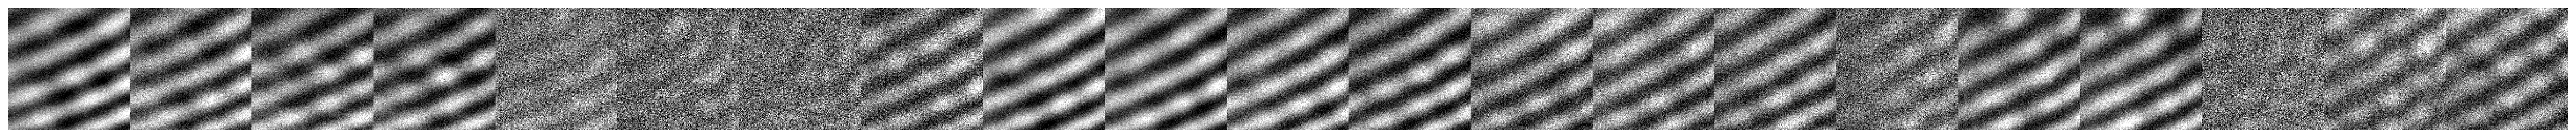
\includegraphics[width=21.1cm]{vortex/sbs.eps}
 }

 \rput[l]{90}(-45,8.5){\parbox{5cm}{
  \Rnode{A}{} \hskip 0.5cm \Rnode{B}{  Intensity} \ncline[linecolor=red]{A}{B} \\
 }}

 \rput[l]{90}(10,8.5){\parbox{5cm}{
  \Rnode{A}{} \hskip 0.5cm \Rnode{B}{  Contrast} \ncline[linecolor=red]{A}{B} \\
 }}

 \rput[c]{90}(65,0){ring angle (a.u)}

 \end{pspicture}
\end{center}
\caption{Intensity and contrast in a ``vortex'' area.  Contrast is defined
here as the ratio of the range (average of the top \SI{1}{\percent} minus
the average of the bottom \SI{1}{\percent} of the intensity values) divided
by the mean intensity.  Note that in certain dark areas of the ring you can
still still have as much contrast as in some of the the brightest places.
The green dashed line in the intensity plot is the noise threshold. }
\label{fig:vortexcontrast}
\end{figure}

\begin{figure}
\begin{center}
\psset{xunit=1.6711cm,yunit=4cm}
\readdata{\dataa}{primarystripes/cone5.txt}
\readdata{\datab}{primarystripes/acone5.dat}
\begin{pspicture}(0,0)(6.2832,1.5)
 \psaxes[trigLabelBase=2,dx=\psPiH,trigLabels,Dy=0.2]{-}(0,0)(6.2832,1.5)
\listplot[linecolor=red,plotstyle=dots,dotstyle=o]{\dataa}
\psclip{\psframe[linestyle=none](0,0)(6,1.4)}
\listplot[linecolor=blue]{\datab}
\endpsclip
\end{pspicture}
\end{center}
\caption{Primary stripe angle as a function position around the ring:
experiment and theory.  This data was taken from Bert's thesis.}
\label{fig:bertconeangle}
\end{figure}


